\documentclass[11pt,a4paper]{article}
\usepackage{hyperref}


\usepackage{times}
\usepackage[T1]{fontenc}
\usepackage{graphicx}
\usepackage{subfigure}
\usepackage{epsfig}
\usepackage{fancyhdr}
\usepackage[dvipsnames]{color}

\textwidth = 170.0mm
\textheight = 246.0mm

\topskip=5mm
\topmargin=0mm
\evensidemargin=-5.4mm
\oddsidemargin=-5.4mm
\headheight=14pt
\headsep=5mm

\parindent=0mm
\parskip  =2mm

\pagestyle{fancy}

\fancyfoot[C]{}

\voffset=-1.25cm
%\pagenumbering{arabic}
%\setcounter{page}{1}
\headheight=15pt

%\definecolor{mygray}{cmyk}{0,0,0,0.4}
\definecolor{mygray}{gray}{0.5}
\fancyhf{}
\rhead{\textcolor{mygray}{\fontsize{10}{12}\selectfont F1. Name1, F2. Name2}}
\renewcommand{\headrule}{{\color{mygray}%
       \hrule width\headwidth height\headrulewidth \vskip-\headrulewidth}
}%renewcommand headrule

\renewcommand\textfraction{.02}
\renewcommand\floatpagefraction{.98}

% for rule under section heading
\newcommand {\sectionrule}{\vskip -0.9 cm
\color {mygray} \rule [0 cm] {17 cm}{0.1 mm} \color {black}}

%%%%%%%%%%%%% START %%%%%%%%%%%%% 
\date{}

\title{Developments done during Polly Schmederer's ACCORD VS at DMI (June 2024) }

\author{Polly Schmederer (GeoSphere) \\ Carlos Peralta (DMI) \\ Fabrizio Baordo (DMI)}
\date{August 2024}


\begin{document}
\maketitle
\thispagestyle{fancy}
%\begin{flushleft}

\section{Introduction}
\sectionrule
This contribution summarizes the work carried out by Polly Schmederer in contribution with Fabrizio Baordo
and Carlos Peralta during the ACCORD-funded visit of Polly in June 2024.

Generalising spatial verifications: 
\begin{itemize}
    \item improving R scripting;
    \item use of reticulate package to interface R with Python;
    \item generalise/apply harp panel tool ("panelification")\\
    (This is a harp and R based version of the originally Python-based \href{https://github.com/pscheffknecht-geosphere/panelification/tree/main}{panelification}.);
    \item providing examples.
\end{itemize}


This is a style example for contributions for ACCORD Newsletter written in \LaTeX. 


\section{Layout}
\sectionrule

\subsection{Layout of headings}

The headings of main sections are underlined. This is achieved by the new command "sectionrule".

\subsection{Table layout}

An example of a Table is given in \ref{tab:grib}. Please feel free to make a more fancy one if you like.

\begin{table}
{\center\it\caption{ \label{tab:grib}Extract of the GRIB header section 1}}
\begin{center}
\begin{tabular}{lrr}
                                        & HIRLAM & ECMWF \\
 Parameter identifier (Code Table 2).   &   122  & 146 \\
 Type of level (Code Table 3).          &   105  &   1 \\
 Time unit (Code Table 4).              &     1  &   1 \\
 Time range one.                        &     0  &   6 \\
 Time range two.                        &     6  &   0 \\
 Time range indicator (Code Table 5)    &     4  &   0 \\
\end{tabular}
\end{center}
\end{table} 

\subsection{Figure layout}
Figures have to be provided in high resolution, preferably in Encapulated PostScript (eps) format, or ".png", ".jpg" or ".gif". 
\textbf{Please, NO .PS files (PDFLaTeX cannot use .ps image files to produce a .pdf file).}
In principle it is best to provide me seperately the image files that are closest to the creating source and have not yet been converted into another format.

The picture caption is placed under the picture, in italic, for example see Figure \ref{fig:O3}.

Please be careful with the size of your picture. LibreOffice has tools to reduce the size of the .pdf file created from your article (with reducing the definition of the pictures). It's not the case with latex (or I don't know how to do that), thus the pictures you provide should have reasonable size.

\begin{figure}[ht] %[h*]
\begin{center}
  \centerline{
   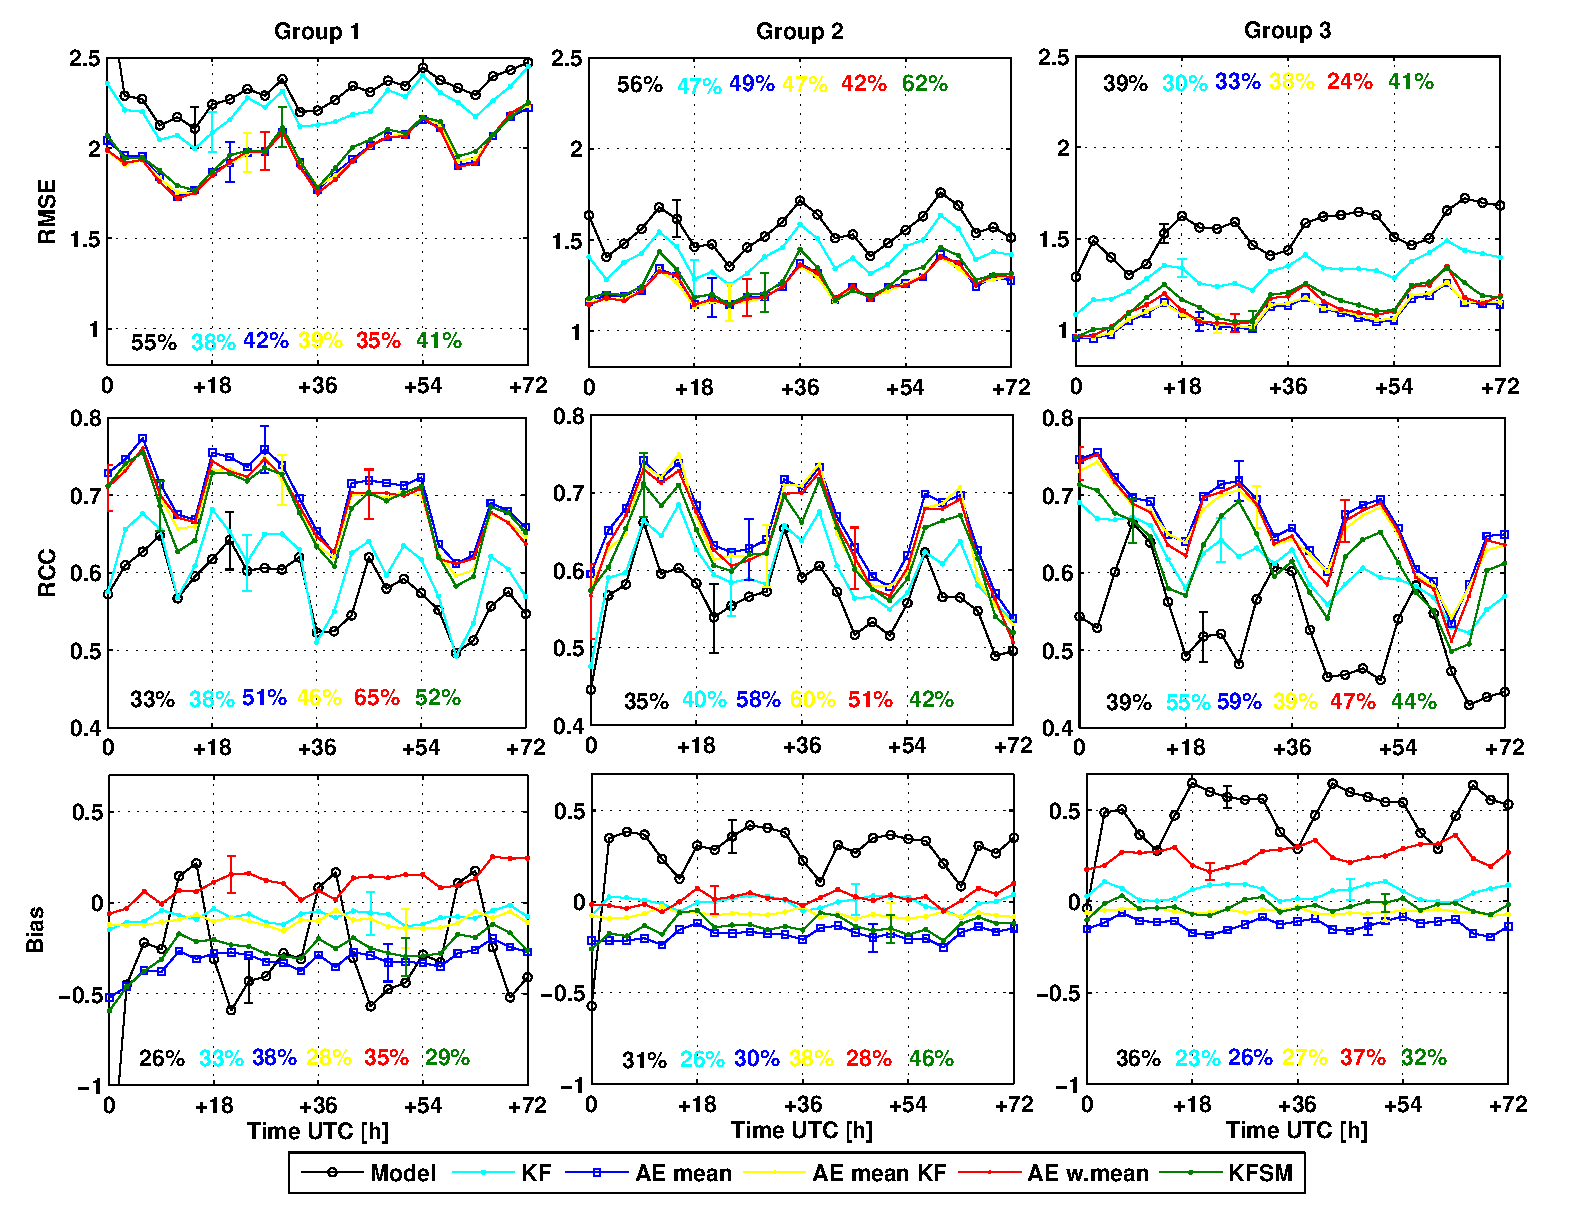
\epsfig{file=./exemple.eps,scale=0.6}
  }
\end{center}
  {\center\it\caption{\label{fig:O3}
   Title of my figure}}
\end{figure}



\section{References}


Bessagnet B., A.Hodzic, R.Vautard, M.Beekmann, S.Cheinet, C.Honor\'e, C.Liousse and L.Rouil,
Aerosol modeling with CHIMERE - preliminary evaluation at the continental scale, Atmospheric
Environment, 38, 2803-2817, 2004.



%\end{flushleft}
\end{document}

 
